\documentclass[20pt]{beamer}
\usepackage[]{bookmark}
\usepackage[utf8]{inputenc}
\usepackage{amsmath}
\usepackage{amsfonts}
\usepackage{amssymb}
\usepackage{tikz}
\usepackage{xcolor}
\usepackage[dutch]{babel}
\usepackage{sansmathaccent}
\usepackage{graphicx}

\pdfmapfile{+sansmathaccent.map}

\title{Recursieve Monte Carlo}
\author{Isidoor Pinillo Esquivel }
\usetheme{Madrid}
\date{}

\begin{document}

\begin{frame}
    \titlepage
\end{frame}


\begin{frame}
    \frametitle{focus}
    \begin{itemize}
        \item recursieve integraal vergelijkingen
        \item ODEs
        \item PDEs
    \end{itemize}
\end{frame}

\begin{frame}
    \frametitle{voorbeeld}
    \vspace{-2cm}
    \action<+->{}
    \begin{align}
        \action<+->{y'   & =y  }                        \\
        \action<+->{y(t) & =y(0)+ \int_{0}^{t} y(s)ds } \\
        \action<+->{Y(t) & =y(0)+tY(S) } \label{RRVE}
    \end{align}

    \action<+->{$S \sim \text{Uniform}(0,t)$}
\end{frame}

\begin{frame}
    \frametitle{voorbeeld}
    \vspace{-2cm}
    \action<+->{}
    (\ref{RRVE})+
    \begin{itemize}
        \action<+->{\item recursie in recursie}
              \action<+->{\item (lineaire) control variates }
              \action<+->{\item Russische roulette}
    \end{itemize}
\end{frame}

\begin{frame}
    \frametitle{loglog plot}
    \begin{center}
        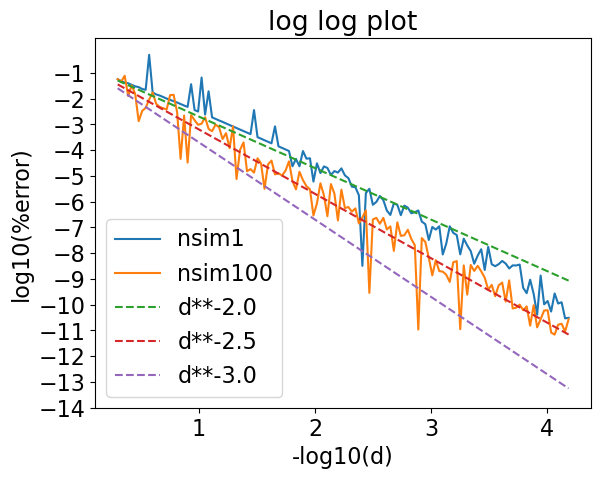
\includegraphics[width=0.8\textwidth]{llplot.png}
    \end{center}
\end{frame}

\begin{frame}
    \frametitle{wanted list}
    \begin{itemize}
        \item stabilisatie IVP solver
        \item hogere orde $1$D BVP solver
        \item WoS warmte vergelijking
    \end{itemize}
\end{frame}

\end{document}